\section{\cp}
\label{sec:CPV_CP}
 \cp\ is simply the combined operation of \cs\ and \ps.
 For \cp\ eigenstates (only neutral particles can be \cp\ eigenstates, or
 systems of particles with overall zero charge), \cp\ is simply
 calculated by multiplying the $C$ and the $P$ quantum numbers.

 Applying the rules for \cs\ and \ps quantum numbers from the
 previous section this means for systems of particles:
\begin{itemize}
\item For a system of \cp\ eigenstates the total \cp\ number is given my
  multiplying the intrinsic \cp\ quantum numbers of the particles
  involved, times a factor $(-1)^L$.
\item A particle-antiparticle pair of bosons has the \cp\ eigenvalue
  $+1$, and a fermion-antifermion pair $(-1)^{S+1}$.
\end{itemize}


\subsection{Time Reversal and the \cpt\ theorem}
 The operation of time reversal reversed the direction of motion,
 i.e. it is as if you would run the movie backwards. The combined
 symmetry \cpt\ is believed to be a good symmetry of any sensible theory
 for rather fundamental reasons (I think it's causality and Lorentz
 invariance this is based on). \cpt\ violation would be big news,
 because it's certainly not expected.

 This means that one can usually consider \cp\ violation equivalent to
 \ts\ violation.

\section{Discovery of \cp\ violation}

 It is easy to see why, from what we have seen so far, \cp\ seems like a
 good candidate for good symmetry. We found that the requirement that
 only chirality left-handed particles participate in the weak
 interaction has the effect that helicity-left-handed particles
 and helicity-right-handed antiparticles take part. Parity
 transforms left and right handed helicity, and charge conjugation
 transforms particles to antiparticles, so under \cp\ we transform a
 helicity left-handed particle into a helicity right-handed
 antiparticle, so something that interacts weakly to something that
 still interacts weakly. Exactly in the same way? We'll see - in many
 cases yes, but in general, no.


 Originally it was hoped that \cp\ symmetry would replace the 'lost'
 \ps\ symmetry, and it came as a surprise when in 1964 Cronin and Fitch
 discovered that \cp\ was in fact violated in the neutral Kaon
 system\cite{cpdiscovery}.

 As opposed to the neutral pion, the neutral Kaon is not its own
 antiparticle. In fact the koans mix (see later) to form two distinct
 \cp\ eigenstates with well-defined (and different) mass and lifetime (at least in the absence of \cp\ violation):
 \begin{align}
 \label{eq:KaonCPevenOdd}
  \ket{K^0_{\mathsf{CP-even}}} &= \frac{1}{\sqrt{2}}\left(\ket{K^0} + \ket{\overline{K}^0}\right)
   &
  \ket{K^0_{\mathsf{CP-odd}}} &= \frac{1}{\sqrt{2}}\left(\ket{K^0} - \ket{\overline{K}^0}  \right)
 \end{align}
 The \cp\ even state decays into two pions (that's how we know it's \cp\ even) while the \cp\ odd state has to decay to three pions to conserve \cp\, meaning far less phase space and a longer lifetime.
 These states are therefore referred to as "K-short", \prt{K_S^0}, 
 and "K-long", \prt{K_L^0}.

 In 1964, Cronin and Fitch discovered that the supposedly \cp\-odd
 \prt{K_L} sometimes decays to two pions, and thus \cp\ is violated
 \ref{cpdiscovery}. 
 It means that the mass eigenstates (i.e. the eigenstates of the Hamiltonian), 
 \prt{K_S^0} and \prt{K_L^0} 
 cannot anymore be identified with the \cp\ eigenstates in \eqnref{eq:KaonCPevenOdd}. 
 It means that in this sytem $[H,CP] \neq 0$, hence \cp\ is violated.

 Now we have two subjects to cover, which will finally lead us to B
 mesons and mixing. One is mixing of neutral particles (like neutral
 Kaons or B mesons). The other is also called mixing but refers to the
 quark-mixing matrix. This is important because this is where \cp\
 violation in the Standard model occurs. This is where we
 start.


\section{Quark Mixing and \cp\ violation}

 Now we finally connect the two seemingly disparate subjects we just
 treated, \cp\ violation and quark mixing.

 The logic is the following: \cp\ violation is observed in weak decays of
 quarks. Weak decays of quarks are governed by quark mixing. \cp\
 violation is due to quark mixing?

\subsection{Quark transitions under \cp\ and \ts}
 As we established above, the transition amplitudes of quarks are
 proportional to the relevant mixing matrix element. So, apart from a
 common factor, the matrix elements of the mixing matrix are the
 transition amplitudes of the quarks. It is convenient to write the
 mixing matrix in the following way:
\begin{equation}
 \vII{d^{\prime}}{s^{\prime}} =
 \mII{V_{ud}}{V_{us}}
     {V_{cd}}{V_{cs}}
 \vII{d}{s}
\end{equation}
  This is the same equation as before, just written in a different,
  convenient notation.

\paragraph{Down to Up transitions}
  With this notation, a $d\to u$ transition has an
  amplitude $V_{ud}$, a $s \to u$ transition an amplitude $V_{us}$,
  etc (all to be multiplied by a common factor that we will ignore).

\paragraph{Up to Down, or the effect of \ts}
  Transitions in the other direction (from u-type to down-type quarks)
  have the complex-conjugate amplitude, so $u\to d$ has the amplitude
  $V^{*}_{ud}$ and $c\to d$ has the amplitude
  $V^{*}_{cd}$, etc. Note that this is not true for amplitudes in
  general, but it is for mixing matrix elements. This result does not
  follow from what we have done in the preceding section, and a
  derivation would be beyond the scope of this lecture, so we just
  state it.

\paragraph{The effect of \cp}
  \cp\ conjugation is equivalent to complex-conjugating the mixing
  matrix element, so $\bar{d} \to \bar{u}$ transitions have amplitude
  $V^{*}_{ud}$, etc. Again, we just state this result w/o any further
  justification, except for mentioning that we could have guessed this
  from \cpt\ symmetry and the previous paragraph. Note that this is
  for \cp\ conjugation - \cs\ conjugation alone would have a different
  effect, the transition amplitude would be zero (it is weak
  interaction after all), it must be \cp. Here we assume that we are
  dealing always with chirality left-handed quarks.

Hence...
\textbf{To put \cp\ violation in mixing we need complex mixing matrix
  elements.}

\fbox{\parbox{0.98\textwidth}{\label{box:CKMVertices}
    \textbf{Associating quark mixing (CKM) matrix elements to vertices in Feynman diagrams:\\}
    \begin{tabular}{cccc}
    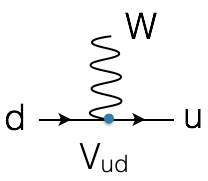
\includegraphics[width=0.18\textwidth]{fig/C_P_CP/Vud_d2u}
    &
    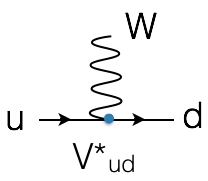
\includegraphics[width=0.18\textwidth]{fig/C_P_CP/Vud_u2d}
    &
    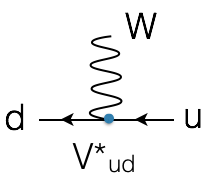
\includegraphics[width=0.18\textwidth]{fig/C_P_CP/Vud_antid2u}
    &
    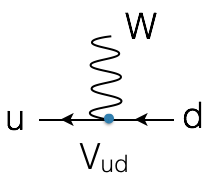
\includegraphics[width=0.18\textwidth]{fig/C_P_CP/Vud_antiu2d}
    \end{tabular}\\
    In the above example you can replace $d$ with any down-type quark (i.e. $s, b$) and $u$ with any up-type quark (i.e. $c, t$). E.g.:\\ 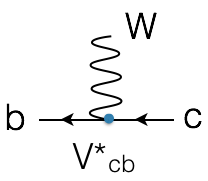
\includegraphics[width=0.18\textwidth]{fig/C_P_CP/Vcb_antib2c}.
}}

\subsection{A closer look at mixing *}
 Now so far, our Cabibbo mixing matrix only has real elements. Maybe
 one of them is in fact complex, thus explaining the observed \cp\
 violation in the Kaon system?

 Let us first look at the constraints that exist on the Cabibbo
 matrix. We view it as a basis transformation, transforming the mass
 eigenstates ($d,s$) to the weak-interaction partners of the $u$ and
 the $c$ quark, $d^{\prime}, s^{\prime}$. For such a
 transformation, we demand that the length of the state vector does
 not change - i.e. we don't get more quarks, for fewer, after the
 transformation than before.
 Mathematically this means:
\begin{eqnarray}
 \vII{d^{\prime}}{s^{\prime}}^{\dagger}
 \vII{d^{\prime}}{s^{\prime}}
=
 \left( V \vII{d}{s}\right)^{\dagger}
  V \vII{d}{s}
&=&
 \vII{d}{s}^{\dagger}
 V^{\dagger} V
 \vII{d}{s}
\nonumber\\
&=&
 \vII{d}{s}^{\dagger}
 \vII{d}{s}
\end{eqnarray}
 where $\dagger$ stands for ``Hermitian conjugate'', i.e. transposed
 and then complex-conjugated.  Since the above expression must be true
 for any $d,s$ vector, this implies for the mixing matrix $V$:
\begin{equation}
 V^{\dagger} V = 1
\end{equation}
 In words: \textbf{$V$ must be a unitary matrix}. In fact, this is all
 that theory predicts about $V$.

\subsubsection{Phases in a $2\times 2$ mixing matrix *}
 A general $2\times2$ unitary matrix can be parameterised by one
 (real) angle, and three complex phases. Now that looks like good news
 - complex phases is what we wanted. But not all complex phases are
 physically meaningful, as we know from basic quantum mechanics. If we
 remove all 'arbitrary' phases, and still are left with a complex
 phase in the mixing matrix, then we actually have a complex mixing
 matrix element where the fact that $V_{ij}^* \neq V_{ij}$ under \cp\
 actually has measurable consequences.

 So what are those arbitrary phases? Essentially each phase in the
 definition of a quark wave function. Now in the entire theory, this
 sort of thing can only be done once - once you've made use if this
 freedom to define the phases of the quark wavefunction, you can't do
 it again. But, take it on trust, no-where else in the Standard Model
 has this freedom yet been exploited, so we can do it here.

 Since the elements of the mixing matrix only appear sandwiched
 between quark wave functions, we can re-define the phases of those
 quark wave functions to remove phases from the mixing matrix.

 There is one phase for each quark field. One of them can be removed
 without having an effect, by removing one over-all phase. This
 over-all phase does not affect the mixing matrix because the
 mathematical expressions in which the mixing matrix appears when we
 calculate transition amplitudes are of the form $u^* V d$, i.e. one
 quark function always enters as the complex conjugate (as usual, in
 matrix elements). If you add an over-all phase to the d and the $u$,
 it'll get cancelled in the expression above since it enters with the
 opposite sign in the $u^*$. It is the old thing that phase
 differences matter, but not the overall phase. What matters are the
 relative phases of the quarks, and of those we have $3$ for a theory
 with 4 quarks, or more generally:

 \textbf{For $n$ quarks we can remove $n-1$ phases from the mixing
 matrix} by fixing the otherwise arbitrary relative quark phases.

 We only had three complex phases in our $2\times 2$ unitary matrix in
 the first place, so we can remove all complex phases of the quark
 mixing matrix, and our mixing matrix is real and determined by one
 parameter - the one we already know, the Cabibbo angle. To summarise
 the important result of this section:

\textbf{For two generations of quarks, there is no room for \cp\
 violation in quark mixing.}

\section{CKM and 3 Generations}

 While everyone realised that \cp\ violation could not be accommodated
 in 2-generation quark mixing, it was M. Kobayashi T. Maskawa who
 realised that this could imply that there are in fact 3 generations
 \cite{progtp.km}.

 Let us do the same counting exercise again that we did above, but now
 for 3 generations, 6 quarks. Now we have a $3\times 3$ unitary
 matrix. This has 9 complex entries, i.e.~18 parameters. The unitarity
 condition provides 9 constraints, leaves 9 free parameters for a
 generic unitary $3\times 3$ matrix. These can be taken as three real
 angles (e.g. Euler angles parameterising real rotations), plus 6
 complex phases.

 With three generations of quarks we have 6 quarks, so we can
 re-define $6-1=5$ relative quark phases to remove complex phases from
 the mixing matrix.
%
 This leaves us with one irremovable, meaningful complex phase. We have
 no prediction for its value, but it \emph{could} parametrise \cp\
 violation. 
%
 Note that, with this, Kobayashi and Maskawa predict the existence of
 an entire generation of new particles (at least 2 quarks, and then
 presumably, for symmetry, 2 leptons) from the observation of \cp\
 violation in Kaon decays, which involve Kaons and pions, made from
 $u,d,s$ quarks, i.e. quarks from only 2-generations.

 All of the predicted particles were subsequently found. The new
 quarks are the bottom quark, discovered in 1977
 \cite{beautydiscovery}, and the very heavy top quark, discovered in
 1994 \cite{topdiscovery}.

 But the real test of the KM theory is not just the existence of a
 third generation, but that \textbf{\cp\ violation is parametrised by
 a single complex phase} in the quark mixing matrix. The $3\times 3$
 quark mixing matrix is called the CKM matrix, after Cabibbo,
 Kobayashi and Maskawa.

 Our quarks are:
\begin{equation}
\vII{u}{d^{\prime}},\;\; \vII{c}{s^{\prime}},\;\; \vII{t}{b^{\prime}}
\end{equation}
 with
\begin{equation}
\vIII{d^{\prime}}{s^{\prime}}{b^{\prime}} = V_{CKM}\vIII{d}{s}{b}
\end{equation}

% And the CKM matrix can be parametrised as
%\begin{equation}
%\label{eq:th.b.vckmpara.pdg}
%V_{\mathrm{CKM}}=
%\mIII{ c_{12}c_{13}    }{
%                    s_{12}c_{13}       }{
%                                  s_{13}e^{-i\delta_{13}} }{
%     -s_{12}c_{23}-c_{12}s_{23}s_{13} e^{i \delta_{13}} }{
%             c_{12}c_{23}-s_{12}s_{23}s_{13}e^{i \delta_{13}} }{
%                     s_{23}c_{13}}{
%     s_{12}s_{23}-c_{12}c_{23}s_{13}e^{i \delta_{13}}}{
%             -c_{12}s_{23}-s_{12}c_{23}s_{13}e^{i \delta_{13}}}{
%                     c_{23}c_{13} }
%\end{equation}\\
% with the three real angles $\theta_{12}, \theta_{13}, \theta_{23}$
% and the complex phase $\delta_{13}$, were we used the short-hand
% notation $c_{ij}=\cos{\theta_{ij}}$ and
% $s_{ij}=\sin{\theta_{ij}}$ for $i,j=(1,2), (1,3), (2,3)$ to fit it
% all in.
\section{The structure of the CKM matrix}
 Let us label the elements of the CKM matrix in a way analogous to the
 Cabibbo matrix earlier:
\begin{equation}
\label{eq:th.b.ckmlabel}
V_{\mathrm{CKM}}=\mIII{ V_{ud} }{ V_{us} }{ V_{ub} }{
                        V_{cd} }{ V_{cs} }{ V_{cb} }{
                        V_{td} }{ V_{ts} }{ V_{tb} }
.
\end{equation}
 Then the transition amplitude from a \qrk{d} to a \qrk{u} quark is
 proportional to $V_{ud}$, the transition amplitude from a \qrk{u} to
 a \qrk{d} quark to $V_{ud}^{\ast}$, etc.

 Experimentally, it is found that the magnitudes of the CKM matrix
 elements follow a clear structure. In terms of the sine of the
 Cabibbo angle, $\lambda\equiv \sin\theta_C=0.22$, the CKM matrix is (very) approximately:
\begin{equation}
\label{eq:ckmLambda}
\mIII{ 1 }{\lambda}{\lambda^3 e^{-i\gamma}}{
      -\lambda}{1}{\lambda^2}{
      \lambda^3 e^{-i\beta}}{-\lambda^2}{1}
.
\end{equation}\\
 Note that this striking structure is not predicted by the Standard
 Model - it is however allowed.  This observation led Wolfenstein to a
 parametrisation of the CKM matrix as a power series in the parameter
 $\lambda$, which is, up to \order{\lambda^3}, given by
 \cite{wolfenstein}: {\small
\begin{equation}
\mIII{ 1-\half \lambda^2    }{ 
                   \lambda                }{ 
                        A\lambda^3\left(\rho-i\eta\right) }{
       -\lambda             }{ 
                    1-\half \lambda^2     }{ 
                        A \lambda^2                        }{
      A\lambda^3\left(1-\rho-i\eta\right)}{
                    -A \lambda^2      }{
                        1                                  }
.
\end{equation}}\\
 where $A, \rho, \eta$ are real parameters of order $1$. The \cp\
 violating phase is parametrised by $\eta$. Up to \order{\lambda^3},
 the only complex elements in this parametrisation are $V_{td}=|V_{td}|e^{-i\beta}$ and
 $V_{ub}=|V_{ub}|e^{-i\gamma}$, where $\gamma \approx 68^o$ and $\beta = 21^o$ (if you include higher order terms, additional CKM matrix element acquire - small - complex phases).
 Putting in some measured values:
 \begin{equation}
\label{eq:th.b.ckmlabel_1}
  V_{\mathrm{CKM}}=\mIII{ V_{ud} }{ V_{us} }{ V_{ub} }{
                        V_{cd} }{ V_{cs} }{ V_{cb} }{
                        V_{td} }{ V_{ts} }{ V_{tb} }
\approx
                 \mIII{ 0.97 }{ 0.23 }{ 0.0037\cdot e^{-i \gamma} }{
                        -0.23 }{ 0.97}{0.041 }{
                        0.0087\cdot e^{-i \beta} }{-0.041 }{0.9991 }
\end{equation}
where $\gamma \approx 68^o$ and $\beta = 21^o$. Don't worry about all the different version of the CKM matrix given here. It is this last version that we will use (and that's given in the formula sheet). But have a look at the others, it helps appreciate the rather striking (near diagonal) structure of the matrix.

For the eagle eyed among you, you must be wondering given the form of
the CKM matrix in Eq.~\ref{eq:ckmLambda} there should be no
\cp\ violation in the Kaon sector as discussed in the previous
section. Indeed this is a subtle point that goes beyond the scope of
this course but you can find an interesting discussion in 
Appendix~\ref{sec:cpv_kaon}.  Basically \cp\ violation in
the Kaon sector enters as a higher order effect in the CKM matrix.

\subsection{Where to look for \cp\ violation}
 Looking at the CKM matrix, we see that the only potentially large
 complex phases are in the top right corner and the bottom left. We
 therefore want decays that involve $b\to u$ transitions or $t\to d$
 transitions. First of all, and this doesn't surprise us after the
 preceding discussion, this means we want decays of quarks from the
 third generation.

 Clearly, $b \to u$ transitions we get from decays of $B$-hadrons,
 which is the generic terms for hadrons involving $b$
 quarks. Interestingly, $t \to d$ transitions are also accessible in a
 certain, rather common species of B hadrons, the \Bdo\ mesons. Where
 and how will be discussed later in the section on B mixing.


\subsection{Unitarity Triangles}
\label{sec:th.b.triangles}
The requirement that the CKM matrix is unitary:
\begin{equation}
\Vckm \Vckm^{\dagger} = \mathbf{1}
\end{equation}\\
 leads to 9 conditions, which are automatically fulfilled in any
 of the above parameterisations. Six of them can be expressed in
 so-called unitarity triangles, which are three complex numbers adding
 up to zero displayed in the complex plane. Below, the six unitarity
 relations leading to the six triangles are listed, together with an
 indication of the length of each side in orders of $\lambda$: {\small
\begin{equation}
\label{eq:CKMUnitarity}
\begin{array}{l c c c c c c c}
1)&V_{ud}^{\ast}V_{us}&+&V_{cd}^{\ast}V_{cs}&+&V_{td}^{\ast}V_{ts}&=&0\\
  & \order{\lambda}   & &\order{\lambda}    & & \order{\lambda^5} & & \\
  &                   & &                   & &                   & & \\
2)&V_{cd}^{\ast}V_{ud}&+&V_{cs}^{\ast}V_{us}&+&V_{cb}^{\ast}V_{ub}&=&0\\
  & \order{\lambda}   & &\order{\lambda}    & & \order{\lambda^5} & & \\
  &                   & &                   & &                   & & \\
3)&V_{us}^{\ast}V_{ub}&+&V_{cs}^{\ast}V_{cb}&+&V_{ts}^{\ast}V_{tb}&=&0\\
  & \order{\lambda^4} & &\order{\lambda^2}  & & \order{\lambda^2} & & \\
  &                   & &                   & &                   & & \\
4)&V_{cd}^{\ast}V_{td}&+&V_{cs}^{\ast}V_{ts}&+&V_{cb}^{\ast}V_{tb}&=&0\\
  & \order{\lambda^4} & &\order{\lambda^2}  & & \order{\lambda^2} & & \\
  &                   & &                   & &                   & & \\
5)&V_{ud}^{\ast}V_{td}&+&V_{us}^{\ast}V_{ts}&+&V_{ub}^{\ast}V_{tb}&=&0\\
  & \order{\lambda^3} & &\order{\lambda^3}  & & \order{\lambda^3} & & \\
  &                   & &                   & &                   & & \\
6)&V_{ub}^{\ast}V_{ud}&+&V_{cb}^{\ast}V_{cd}&+&V_{tb}^{\ast}V_{td}&=&0\\
  & \order{\lambda^3} & &\order{\lambda^3}  & & \order{\lambda^3} & & \\
  &                   & &                   & &                   & & \\
\end{array}
\end{equation}}\\
 If there is no \cp\ violation, the triangles all degenerate to
 lines. Describing \cp\ violation in terms of unitarity triangles has
 the advantage that changing the parametrisation of the CKM matrix,
 and hence the phase-convention for the quarks, simply rotates the
 whole triangle in the complex plane, but leaves the side lengths and
 the relative angles inside the triangle unchanged. Therefore the
 unitarity triangles are a convention--independent way of parameterising
 \cp\ violation in the \sm.

%% The area of the all unitarity triangles is the same and is the
%% geometric, convention-independent equivalent of the single complex
%% phase in the CKM matrix \cite{Jarlskog:triangle_area}:
%%\begin{equation}
%%\mbox{Area of all triangles} = \half \left|J\right|
%%\end{equation}\\
%%with
%%\begin{equation}
%%J=\sum_{m,n=1}^3 \epsilon_{ikm}\epsilon_{jln} 
%%  \Imag\!\left( V_{ij} V_{kl} V_{il}^* V_{kj}^* \right)
%%\end{equation}
%%\begin{displaymath}
%%\mbox{ for any } i,j,k,l \in \left\{1,2,3\right\}
%%\end{displaymath}

\subsection{\emph{The} Unitarity Triangle and the Angles \gam, \bet}
\label{sec:th.b.thetriangle}
 Most of the triangles have very unequal sides. To measure \cp\
 violation in decays related to such triangles, for example in the
 \prt{K^0} system associated to triangle number 1, is very difficult:
 the two long sides have little relative phase difference and
 therefore little \cp\ violating effects; the third short side might have a
 large phase difference relative to the long sides, but this angle is
 then not very well constrained anymore by the length of the other
 sides - a small error on one of the long sides corresponds to a
 relatively large error on the angle ($\propto 1/\mbox{(length of
 short side)}$), and the most appealing feature of the unitarity
 triangles is in fact that it relates \cp\ violating phases to other
 measurements in quark decays and thus tests the SM model.


 Only in the last two triangles are all sides of the same order of
 magnitude. Both are related to observables in decays of neutral \prt{B}
 mesons: number $5$ to \Bso\ decays and number $6$ to \Bdo\ decays. Up
 to \order{\lambda^3} in the Wolfenstein parametrisation, the two
 triangles coincide. Therefore triangle number 6 is called \emph{The}
 Unitary Triangle.
\begin{figure}
\caption{\emph{The} Unitary Triangle\label{fig:th.b.triangle}}
\setlength{\unitlength}{1.2cm}
\begin{picture}(7,2.2)

\put(6,0){\vector(-1,0){5}}
\put(1,0){\vector(1,1){2}}
\put(3,2){\vector(3,-2){3}}

%\put(3,1.5){\mbox{$\alpha$}}
\put(1.5,0.15){\mbox{$\gamma$}}
\put(5,0.15){\mbox{$\beta$}}

\put(5,1){\mbox{$V_{tb}^{\ast} V_{td}$}}
\put(0.3,1){\mbox{$V_{ub}^{\ast} V_{ud}$}}
\put(3,0.15){\mbox{$V_{cb}^{\ast} V_{cd}$}}
\end{picture}
\end{figure}
 This is shown in figure \ref{fig:th.b.triangle}, where also the
 angles \gam\ and \bet\ are defined. The angles \bet\ and \gam\ are the complex phases of the only complex CKM matrix elements (up to $\order{\lambda^3}$, $V_{td}=|V_{td}|e^{-i\beta}$ and $V_{ub} = |V_{ub}|e^{-i\gamma}$. The parameter $\alpha$ that is
 often found in the literature, corresponds to the third angle in figure
 \ref{fig:th.b.triangle}; $\alpha \equiv \pi-\bet-\gam$ (but there is no CKM element with phase $\alpha$. Because \order{\lambda^3}, \bet\ and
 \gam\ are the only non-zero phases in the CKM matrix, and only decays
 involving \qrk{b \to u} or \qrk{d \to t} transitions can violate \cp.
 Both are accessible in the \Bdo\ system, $\gamma$ and other
 interesting parameters are also accessible in the \Bso\ system.

 The unitarity triangle is a convenient way to relate \cp\ violation
 measurements to other measurements in the Standard Model. Non
 \cp-violating measurements of quark transition rates measure the
 absolute size of CKM elements, and hence the length of the sides of
 the triangle. \cp\ violation measurement measure the angles.

 Any inconsistency in these measurements would indicate a failure of
 the Standard model and be a much sought-after hint of new physics.

\subsection{Summary: \cp\ Violation in the Standard Model}
 \begin{itemize}
 \item In the Standard Model, \cp\ violation is parametrised by a
 single complex phase in the CKM matrix. The SM is therefore very
 predictive wrt \cp\ violation.
 \item There are two elements in the CKM matrix with large complex
 phases, these are $\beta$ and $\gamma$ and both depend on the
 previously mentioned single phase. Both are accessible in the B
 system.
 \item The SM predicts that the CKM matrix is unitary.
 \item The Unitarity triangle relates CP-violating phases to other
 measurements, for example absolute transition rates that measure the
 lengths of the side of the unitarity triangle. Any inconsistency
 would indicate new physics.
\end{itemize}
\clearpage
\section{Neutral Meson Mixing/Oscillations}
A phenomenon that is not in itself \cp\ violating, but that is, as we will see in \secref{sec:CPVinB}, closely related, is the phenomenon of meson anti-meson mixing. It is the fascinating property of neutral Kaons ($\overline{s}d$), neutral D-mesons ($c\overline{u}$) and neutral B mesons ($\overline{b}d$) to turn into their own antiparticles and back. This phenomenon is also called "oscillation" because the Meson oscillates between two states, one of which is the antiparticle of the other.\\
\exercise{
Quick question: Why do \piz\ mesons not oscillate?\\
\rotatebox{180}{Because they are their own antiparticle}
}\\

\subsection{Meson mixing in the absence of \cp\ violation}
The discussion below will be applicable to any neutral meson system, we'll use the \Bo, \Bob\ system as an example.

\subsubsection{The two-states \Se\ for the neutral meson system*}
\label{sec:details}
The \Se\ for a superposition of flavour eigenstates, $ a \ket{\Bo} + b
\ket{\Bob}$, is:
\begin{equation}
\label{eq:th.a.se}
%
i\dbyd{}{t}\vII{a}{b}= \op{H} \vII{a}{b}.
%
\end{equation}\\
 

 It can be shown that \cpt\ invariance implies that the diagonal elements of \op{H} are the same and \op{H} and therefore be written as:
\begin{equation}
\op{H}=\mII{h_{11}}{h_{12}}{h_{21}}{h_{11}}.
\end{equation}
The crucial bit are the off-diagonal elements. They make matrix elements like this $\bra{\Bo}
\op{H}\ket{\Bob}$ non-zero, so they allow $\Bo\ \to \Bob$ transitions. If we were dealing with charged particles (like \Bp, \Bm), clearly such transitions would not be allowed, and the Hamiltonian would be diagonal. But for neutral mesons like \Bo, \Bob, as well as \Ko, \Kob, and \Do, \Dob, no conservation law is violated in such transitions, and the off-diagonal elements are non zero. You will see a Feynman diagram for such a transition later in the notes. As we will show below, these off-diagonal elements lead to two distinct mass eigenstates with different masses.

 \op{H} has the following eigenvalues:
\begin{equation}
\lambda_{H,L}=h_{11}\pm \sqrt{h_{21}\cdot h_{12}}
\end{equation}
The diagonalised Hamiltonian is:
\begin{eqnarray}
%
\lefteqn{\op{H_d} = \mII{H_H}{0}{0}{H_L} }\nonumber\\
         & &
= \mII{h_{11} + \sqrt{h_{12} h_{21}}\!\!\!}{0}
    {0}{\!\!\!h_{11} - \sqrt{h_{12} h_{21}}}
.
\nonumber\\
\mbox{}
\end{eqnarray}
 The eigenstates of the Hamiltonian (i.e. what we'd call "real" or "physical" particles), are given by:
\begin{equation}
\label{eq:th.a.def_Bl_Bh}
\ket{\prt{B_{H,L}}} = p \ket{\Bo} \mp q \ket{\Bob},
\end{equation}
with $|p|^2 + |q|^2 = 1$ and
\begin{equation}
\frac{q}{p}= -\sqrt{\frac{h_{21}}{h_{12}}}.
\end{equation}\\
The indices $H$ and $L$ stand for "heavy" and "light" mass eigenstate.
 The diagonalised Hamiltonian \op{H_d} is:
 
\op{H} can be written in terms of two Hermitian matrices, \op{M}, and \op{\Gamma}, as
\begin{equation}
\op{H}= \op{M} - \frac{i}{2} \op{\Gamma}
\end{equation}
where \op{M} represents the energy (mass) of the particles, and \op{\Gamma} represents their decay.
(If the particles were stable, \op{\Gamma} would be zero and the Hamiltonian would be Hermitian as one might expect, but since they do decay, we do not represent the full set of available states with \Bo, \Bob, hence the Hamiltonian is not Hermitian, as probability is not conserved - the system can leave our subspace. This is represented by \op{\Gamma}).

The diagonal mass and decay matrices,
 are:
\begin{eqnarray}
\op{M_d}&=&\mII{M_H}{0}{0}{M_L}
        =\mII{\Real\!\left(H_H\right)}{0}{0}{\Real\!\left(H_L\right)}\\
\op{\Gamma_d}&=&\mII{\Gamma_H}{0}{0}{\Gamma_L} 
             =\mII{2\Imag\!\left(H_H\right)}{0}{0}{2\Imag\!\left(H_L\right)}
.
\nonumber\\
\mbox{}
\end{eqnarray}
 The time-dependent solutions of the diagonal \Se\ are:
 \begin{eqnarray}
 \ket{B_H(t)} &=& e^{-iM_Ht} e^{-\half\Gamma_Ht} \ket{B_H(0)} \nonumber\\
 \ket{B_L(t)} &=& e^{-iM_Lt} e^{-\half\Gamma_Lt} \ket{B_L(0)} \nonumber\\
 \end{eqnarray}
 where $\ket{B_H(0)}, \ket{B_L(0)}$ are the solutions at $t=0$.
 The mass- and width difference between the eigenstates is:
\begin{equation}
\Delta\!m = M_H-M_L, \;\;\;
\Delta\!\Gamma=\Gamma_H-\Gamma_L
\end{equation}\\

\subsubsection{B meson oscillations in the absence of \cp\ violation}
\label{sec:bosc}
 In the previous section it was shown that the mass eigenstates
 for the \Bo-system are given by:
\begin{equation}
\label{eq:th.a.def_Bl_Bh}
\ket{\prt{B_{H,L}}} = p \ket{\Bo} \mp q \ket{\Bob},
\end{equation}
with $|p|^2 + |q|^2 = 1$. 
These have different masses and lifetimes (widths). In the absence of \cp\ violation, these states must also be \cp\  eigenstates. This is the case if $p=q=1/\sqrt{2}$ (or $p=-q$, but we pick $p=q$). 
\begin{equation}
\label{eq:th.a.def_Bl_Bh}
\ket{\prt{B_{H,L}}} = \frac{1}{\sqrt{2}} \left( \ket{\Bo} \mp \ket{\Bob}\right)
\end{equation}
This means that \Bh\ is the \cp-odd state:
\begin{eqnarray}
\cp \ket{B_H} & = & \frac{1}{\sqrt{2}} \left( \cp \ket{\Bo} - \cp \ket{\Bob}\right) \nonumber\\
& = & \frac{1}{\sqrt{2}} \left( \ket{\Bob} - \ket{\Bo}\right) \nonumber\\
& = & - \ket{B_H}
\end{eqnarray}
\Bl\ is \cp-even
\begin{eqnarray}
\cp \ket{B_L} & = & \frac{1}{\sqrt{2}} \left( \cp \ket{\Bo} + \cp \ket{\Bob}\right) \nonumber\\
& = & \frac{1}{\sqrt{2}} \left( \ket{\Bob} + \ket{\Bo}\right) \nonumber\\
& = & \ket{B_L}.
\end{eqnarray}
(the naming convention with $H$ and $L$ is only justified because experimentally, we know that the $CP$ odd state is the heavier one, I don't think there's any fundamental reason why this must be so).

Now we want to know what happens if we start at $t=0$ with a definite \Bo\ or \Bob\ state (as they are for example produced in proton-proton collisions at the LHC).
First we write them in therms of \Bh\ and \Bl, where we know the time evolution.
\begin{eqnarray}
\ket{\Bo} &=&  + \frac{1}{\sqrt{2}} \left(\ket{\Bh} + \ket{\Bl}\right)\nonumber\\
\ket{\Bob}&=&  - \frac{1}{\sqrt{2}} \left(\ket{\Bh} -  \ket{\Bl}\right)
.
\end{eqnarray}
%
In the previous (starred, i.e. non-examinable, but still hopefully interesting) section we found:
 \begin{eqnarray}
 \ket{B_H(t)} &=& e^{-iM_Ht} e^{-\half\Gamma_Ht} \ket{B_H(0)} \nonumber\\
 \ket{B_L(t)} &=& e^{-iM_Lt} e^{-\half\Gamma_Lt} \ket{B_L(0)} 
 \end{eqnarray}
 where $\ket{B_H(0)}, \ket{B_L(0)}$ are the solutions at $t=0$.
%
 The wavefunction of a particle created as a \Bo\ at time $t=0$
 develops as:\\
\newcommand{\expheavy}{e^{-i\left(M_H -\frac{i}{2}\Gamma_H \right) t}}
\newcommand{\explight}{e^{-i\left(M_L -\frac{i}{2}\Gamma_L \right) t}}
\newcommand{\expmh}{e^{-i M_H t}}
\newcommand{\expml}{e^{-i M_L t}}
\newcommand{\expthalf}{e^{-\frac{\Gamma}{2}t}}
%
\parbox{0.97\columnwidth}{
\begin{eqnarray}
%
\ket{\Bo(t)}&=&   \frac{1}{\sqrt{2}}\ket{\Bh}\expheavy \nonumber\\
            & & + \frac{1}{\sqrt{2}}\ket{\Bl}\explight 
.
\nonumber\\
\mbox{}
%
\end{eqnarray}}\\
 Until now, the derivation applied to general neutral meson system,
 including Kaons, \prt{\Do}, \prt{B_s^0}, \prt{\Bo}. To make the maths a bit easier, we will now restrict ourselves to the case where $\Gamma_H \approx \Gamma_L \equiv \Gamma$ is a
 good approximation (which it is for \Bo\ mesons, but even where this is not the case, e.g. for Kaons, we still get a good qualitative idea of the the basic principles)\\
\begin{eqnarray}
%
\ket{\Bo(t)} &=&\expthalf \frac{1}{\sqrt{2}} \left\{ \ket{\Bh}\expmh + \ket{\Bl}\expml \right\}
\nonumber \\
 &=& 
\expthalf \frac{1}{2} 
     \left\{ \left( \ket{\Bo}-\ket{\Bob} \right) \expmh
           + \left( \ket{\Bo}+\ket{\Bob} \right) \expml \right\}
\end{eqnarray}
 The probability to detect a particle that was created at time $t=0$ as a \Bo, at a later time $t$ as a \Bob\, is therefore:
 \begin{eqnarray}
%
\lefteqn{\left|\braket{\Bob}{\Bo(t)}\right|^2} \nonumber\\
&=& \left|
\expthalf \frac{1}{2} 
     \left\{ \left( \braket{\Bob}{\Bo}-\braket{\Bob}{\Bob} \right) \expmh
           + \left( \braket{\Bob}{\Bo}+\braket{\Bob}{\Bob} \right) \expml \right\}\right|^2
\nonumber\\
&=& \left|
\expthalf \frac{1}{2} 
     \left\{- \expmh
            + \expml \right\}\right|^2
\nonumber\\
&=&
e^{-\Gamma t} \frac{1}{4} 
     \left| e^{-i M_L} \left(1
               -  e^{-i(M_H - M_L)t}\right)\right|^2
\nonumber\\
&=&
e^{-\Gamma t} \frac{1}{4} \left(
     \left(1 - \cos\left(\Delta m\;t\right)\right)^2 + \sin^2\left(\Delta m\;t\right) 
     \right)
\nonumber\\
&=&
e^{-\Gamma t} \frac{1}{4} \left(
     1 - 2 \cos\left(\Delta m\;t\right) + \cos^2\left(\Delta m\;t\right) + \sin^2\left(\Delta m\;t\right) 
     \right)
\nonumber\\
&=&
e^{-\Gamma t} \frac{1}{2} \left(
     1 - \cos\left(\Delta m\;t\right) \right)
\end{eqnarray}
The same can be done for the probability that a particle created as a \Bo\ at $t=0$ is observed as a \Bo\ at $t$
\begin{equation}
\left|\braket{\Bo}{\Bo(t)}\right|^2 = e^{-\Gamma t} \frac{1}{2} \left(
     1 + \cos\left(\Delta m\;t\right) \right)
\end{equation}
The probability that we observe any particle at all is simply the sum of these: $e^{-\Gamma t}$

Let's put in a few values: at $t=0$, as expected, the probability that the \Bo\ oscillated into its antiparticle is $0$. The probability to observe it as a \Bob\ at time $t = \frac{\pi}{\Delta m}$ is $e^{-\Gamma t}$, while to observe it at $t = \frac{\pi}{\Delta m}$ in the same state in which it was born, as a \Bo, is null. So if I find that the particle has not decayed by that time, the probability that it has turned into its antiparticle is $100\%$! And at $t = \frac{2\pi}{\Delta m}$ we have come full circle, if it survived this long, we'll certainly observe it as \Bo\ again. In between it could be observed in either state\footnote{The way we know if it was a \Bo\ or a \Bob\ is by using final states that are only accessible to one or the other. For example, \Bo\ can decay to $\bar{D}^0 \mu^+ \nu_{\mu}$ while \Bob\ cannot.}

So, in summary, \Bo\ mesons oscillate with a frequency proportional to their mass difference between the \Bo\ and \Bob\ state. 

\subsubsection{The mixing mesons}
\begin{figure}
\centering
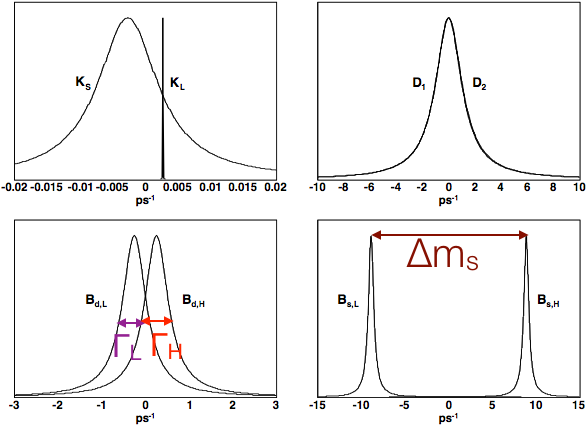
\includegraphics[width=0.7\textwidth]{fig/C_P_CP/MixingMesons}
\caption{Breit Wigner functions describing the lineshapes of the mass eigenstates of mixing neutral mesons systems. The wider the curve, the smaller the lifetime since $\tau = 1/\Gamma$. The peak represents the mass of the particle. The $x$ axis has an offset so that all plots are centred at $0$, so you cannot read off the absolute masses, but you can use it to read off the mass differences and the widths. The units (inverse picoseconds) are a bit unusual, but make it easy to translate this into oscillation frequencies and lifetimes.\label{fig:MixingMesons}}
\end{figure}
Mixing has been observed in Kaons, \Do\ mesons, \Bo\ mesons and \Bso\ mesons. The basic properties (mass and width) of the different meson eigenstates are illustrated in \figref{fig:MixingMesons}. The figure shows the Breit Wigner lineshapes of different mesons. Each lineshape describes the distribution of masses you expect to measure if you observe a large number of particle decays - so there is a mass (energy) uncertainty, represented by the width $\Gamma$ (which is the full width half maximum (FWHM) of these curves). The width is related to the lifetime via $\Gamma = \frac{1}{\tau}$ (or, in SI units, $\Gamma = \frac{\hbar}{c^2\tau}$).  In the plot, the mass is expressed in inverse picoseconds, which might seem a bit peculiar, but given the relationship $\Gamma = \frac{1}{\tau}$, and given that we found earlier that the mixing probability is proportional to $1-\cos\Delta\!m t$, it is quite convenient. The absolute values on the $x$--axis in \figref{fig:MixingMesons} are arbitrary, but the scale is not, so we can read off $\Delta m$ and $\Gamma$.

We observe that for neutral kaons, the most significant difference between the mass/width eigenstates is in the lifetime, which is why we label them by their lifetimes as \Kl\ ("K-long") and \Ks\ ("K-short"). The mass difference is quite small, so they oscillate very slowly. For both \prt{B} mesons, the widths/lifetimes are very similar, hence we label them as $B_H$ ("B-heavy") and \prt{B_L} ("B-light"). The mass difference between the two \Bso\ states is much bigger than between any of the others, so \Bso\ mesons oscillate very fast. It requires excellent time resolution to measure this. \Do\ mesons, both mass and width are nearly (but not quite) the same, so they oscillate extremely slowly, which is also challenging because you need an incredibly large number of \Do\ mesons to see any hint of an oscillation at all. This is why \Bso\ and \Do\ oscillations were discovered much later than kaon and \Bdo\ oscillations.

\subsection{Mixing and GIM suppression}
\begin{figure}[!h]
\begin{tabular}{cc}
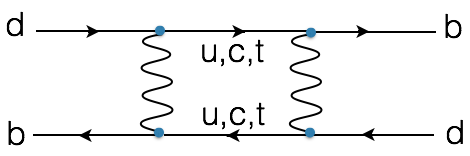
\includegraphics[width=0.4\textwidth]{fig/C_P_CP/BMix1}
&
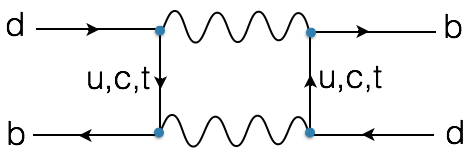
\includegraphics[width=0.4\textwidth]{fig/C_P_CP/BMix2}
\\ a & b
\end{tabular}
\caption{The two box diagrams mediating B mixing.\label{fig:BMixingDiagrams}}
\end{figure}
The Feynman diagrams that allow a \Bo\ to turn into a \Bob\ are given in 
\figref{fig:BMixingDiagrams}.\\
The mixing diagrams such as those for the \Bo\ shown above are clearly flavour changing neutral currents. The same mechanism that suppresses flavour changing neutral currents in the two family model works in principle also with 3 generations of quarks. Instead of $\cos\theta_C$ and $\sin\theta_C$ we now associate the appropriate CKM matrix elements to the vertices, following the rules given in the box on page~\pageref{box:CKMVertices}. For example, we get for the contribution for a loop with two virtual $u$ quark lines: $V_{ud} V_{ub}^* V_{ub}^* V_{ud}$; with two internal $t$ quark lines: $V_{td} V_{tb}^* V_{tb}^* V_{td}$; with a $c$ quark and a $t$ quark: 
$V_{cd} V_{cb}^* V_{td} V_{tb}^*$; etc.
(Note that this is the same for both diagrams shown in \figref{fig:BMixingDiagrams}.) If $u, c, t$ all had identical masses, the sum of the matrix elements would be proportional to the sum of all the relevant products of CKM matrix element. We will now calculate this sum. To make this less messy, we introduce the following notation: $\mathcal{M}_{ij}$ stands for the product of CKM matrix element for the diagram an $i, j$ combination of internal quark lines. We also observe that $\mathcal{M}_{ij} = \mathcal{M}_{ji}$, i.e. for the diagram on the left, you'll find that, in terms of CKM matrix elements it doesn't matter whether the top line is $u$ and the bottom is $\bar{t}$ ($\mathcal{M}_{ut}$) or the top line $t$ and the bottom one $\bar{u}$ ($\mathcal{M}_{tu}$).
\begin{eqnarray}
\lefteqn{\sum\limits_{i=u,c,t}\sum\limits_{j=u,c,t}\mathcal{M}_{ij}}
\nonumber\\
&=& 
\mathcal{M}_{uu} + \mathcal{M}_{cc} + \mathcal{M}_{tt} 
+ 2\left(\mathcal{M}_{uc} + \mathcal{M}_{ut} + \mathcal{M}_{ct}\right)
\nonumber\\
&=& V_{ud}^2 V_{ub}^{*2} 
+ 
V_{cd}^2 V_{cb}^{*2}
+
V_{td}^2 V_{tb}^{*2}
+
2 \left(
V_{ud} V_{ub}^{*}V_{cd} V_{cb}^{*}
+ V_{ud} V_{ub}^{*}V_{td} V_{tb}^{*}
+V_{cd} V_{cb}^{*}V_{td} V_{tb}^{*}
\right)
\nonumber\\ &=&
\left(V_{ud} V_{ub}^{*} 
+ 
V_{cd} V_{cb}^{*}
+
V_{td} V_{tb}^{*}\right)^2
\nonumber\\ &=& 0
\end{eqnarray}
where in the last step, we used the unitarity relations given in Equations~\ref{eq:CKMUnitarity}. 

\exercise{Draw the equivalent Feynman diagrams for Kaon mixing and D meson mixing, and repeat the exercise, i.e. show that if all quark masses were the same, the sum of the mixing diagrams over all internal quark lines would be zero.}

So if all up-type quark masses were the same, the GIM cancellation would work perfectly even in three (or more) generations, as long as the mixing matrix is unitary. But of course the quark masses are not equal.
Especially, the top quark mass is huge (\un{175}{GeV} compared to $0$ ish for the $u$ and few GeV for the $c$ quark). As a consequence, and combined with the large value of $V_{tb}$, the top contribution completely dominates the \Bo--\Bob\ mixing diagram. 
A rough numerical estimate for the different contributions can be obtained by multiplying the approximate magnitude of the CKM elements with the mass of the internal quark.
\begin{itemize}
 \item For the $d \to t \to b$ transition this is is $\sim \lambda^3 m_{t}^{2}$.
 \item For the $d \to c \to b$ transition this is $\sim \lambda^3 m_{c}^{2}$
 \item For the $d \to u \to b$ transition this is $\sim \lambda^3 m_{u}^{2}$
\end{itemize}
 If you now take into account that the top is $\sim 100\times$ as
 heavy as the charm, and $100,000$ times as heavy as the $u$ quark,
 it is clear that the top contribution completely dominates and we can neglect the contributions of the other
 quarks. The same is true for \Bso\ mixing. This will simplify the calculations we'll do with these diagrams, later. For the kaon mixing diagram, the picture is a bit more murky, because $V_{ts}$ is quite small. And for charm mixing, we need to look at GIM cancellation with internal $d, s, b$ quarks, which works better (the range of masses is much more restricted), plus the $b$ quark contributions are suppressed because they involve only small CKM matrix elements. 
The consequence of all of this is that \Bo\ and \Bso\ oscillations are quite fast (especially \Bso
 - they were so fast that it took until 2006 for them to be discovered), while Kaon oscillations are quite slow, and \Do\ oscillations are extremely slow (so slow it took until 2007 for them to be discovered). In fact the measurement of the \Bdo\ oscillation frequency was used to estimate the top mass long before the top had been produced directly.

And why did 2-generation GIM cancellation ever work? Because of the coincidence that the CKM matrix nearly has a $2 + 1$ block structure:
\[
V_{CKM} \sim \parbox{0.2\textwidth}{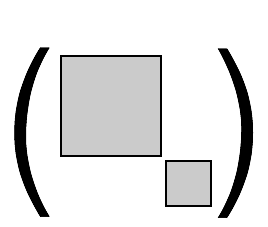
\includegraphics[width=0.2\textwidth]{fig/CKM_block}}
\]
which means that both the $2\times 2$ block and the $1\times 1$ block are approximately separately unitary, to a good enough approximation at least that GIM worked fairly well when it was conceived. But it's important to remember that it's those small off-diagonal elements, which destroy this simple picture, that couple the 3rd generation of quarks to the other two, and are responsible for CP violation.
